\chapter{Sistema de aproximación de la distancia}
\label{cha:Sistema de aproximación de la distancia}

\begin{FraseCelebre}
  \begin{Frase}
    Texto.
  \end{Frase}
  \begin{Fuente}
    Autor texto
  \end{Fuente}
\end{FraseCelebre}

\noindent
Obteniendo las detecciones 2D de los objetos dentro del \ac{FoV} de la cámara utilizada, se procede al estudio de los posibles métodos a utilizar para la aproximación de la distancia a cada uno de los objetos del entorno. Como técnicas a evaluar, en un principio se plantea: el uso de un método basado en una regresión utilizando las características más importantes que consigan predecir la distancia y la obtención directa la distancia mediante la proyección de la nube del puntos del \ac{LiDAR} sobre la cámara del vehículo; siendo ambas técnicas basadas en modelos clásicos de \ac{ML}, todo ello para permitir más adelante la reducción de la \ac{RoI} a analizar, para obtener las detecciones 3D finales.

El estudio y elección de los modelos de aproximación de la distancia se han realizada sobre cuadernos de trabajo Jupyter utilizando el lenguaje Python para simplificar el tratamiento de los datos, además de la necesidad de tratar con imágenes y nubes de puntos dentro de este apartado. Este trabajo se puede encontrar en en siguiente repositorio git alojado en GitHub, dentro de la carpeta 'Distance approximation': \url{https://github.com/Javier-DlaP/3D-detection-system-lidar-camera}.

\section{Análisis del dataset KITTI}
\label{sec:Análisis del dataset KITTI}

El primer paso dentro del proceso de creación de un modelo de \ac{ML} consiste en la comprensión de los datos con los que se está trabajo, por ello, en este primer apartado, se va a observar que datos de importancia aporta KITTI para la creación del modelo requerido.

Dentro del dataset de KITTI el ground-truth se encuentra guardado como un archivo de texto por cada uno de los 7.481 frames de datos guardados. En este ground-truth se observa la aparición de: coches, peatones, ciclistas, camiones y objetos desconocidos; pero ya que dentro del evaluador de KITTI solo se analizan: coches, peatones y ciclistas; se ha decidido estudiar únicamente estas clases \cite{kitti_evaluator_3d}. Con la elección de los datos a utilizar, se genera un script que unifica en un dataframe todos los archivos de ground-truth del dataset para poder analizarlos de forma más sencilla. Tras esto se consigue un dataframe con 34.856 objetos diferentes (únicamente de las clases: coche, peatón y cilista), en el que se recoge por cada objeto la información del: frame, identificador, tipo, visibilidad, rotación, bounding box 2D, dimensiones, centro tridimensional, etc. De forma adicional, se generan varias características extra que se espera que aporten información al estudio como: la distancia a cada objeto, la altura y anchura en píxeles de las bounding boxes 2D, y la completitud de las bounding boxes 2D en la componente vertical y horizontal debido a la aparición de objetos parcialmente visibles debido al \ac{FoV} de la cámara utilizada en este dataset. En cuanto al uso del dataframe para el ajuste y evaluación de los modelos a crear, se ha dividido dicho dataframe creado en dos diferentes, uno de entrenamiento y otro de evaluación atendiendo a la división dada por el dataset de KITTI.

\begin{figure}[H]
    \centering
    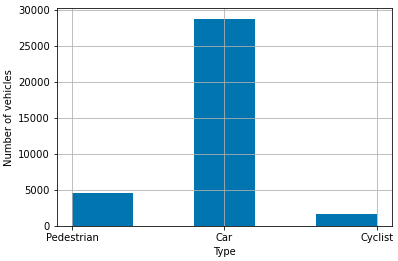
\includegraphics[width=0.4\textwidth]{Book/figures/6_approx_distancia/classes_kitti.png}
    \caption{Aparición de las clases en KITTI.}
    \label{fig:Aparición de las clases en KITTI.}
\end{figure}

Uno de los problemas más importantes a tener en cuenta dentro del dataset de KITTI es la pésima distribución de las clases con las que se trata. Como se observa en la Figura \ref{fig:Aparición de las clases en KITTI.}, en torno a un 80\% de objetos con los que se trabaja son coches por lo que es muy importante tener esto en cuenta, ya que no todas las clases tienen las misma características y puede influir negativamente en el ajuste de los modelos a diseñar. En cuanto a este hecho, la aplicación de técnicas de fine tuning presentadas en el Capítulo \ref{sec:Entrenamiento y evaluación de YOLOv5} para el entrenamiento del modelo de detección del objetos 2D consigue evitar parcialmente el sobreajuste que implica el uso de clases tan desbalanceadas.

\begin{figure}[H]
	\begin{minipage}{0.48\textwidth}
		\centering
		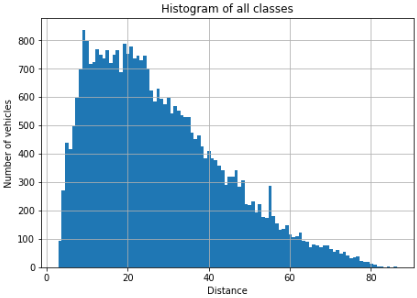
\includegraphics[width=0.97\linewidth]{Book/figures/6_approx_distancia/distance_kitti.png}
		\caption{Distribución de la distancia.}
		\label{fig:Distribución de la distancia.}
	\end{minipage}\hfill
	\begin{minipage}{0.45\textwidth}
		\centering
		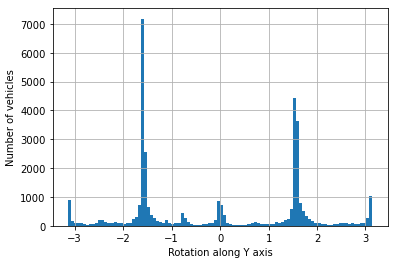
\includegraphics[width=1\linewidth]{Book/figures/6_approx_distancia/rotation_y_kitti.png}
		\caption{Distribución de la rotación.}
		\label{fig:Distribución de la rotación.}
	\end{minipage}
\end{figure}

De la misma que se ha  analizado los datos en relación al tipo de clase presente en el dataset, otras de las características más interesantes para su análisis son: la distribución de distancias a cada objeto del ground-truth y la rotación respecto del eje del propio vehículo del resto de objeto del entorno.

La Figura \ref{fig:Distribución de la distancia.} muestra la distribución de la distancia a los vehículos del ground-truth calculada como la distancia desde el origen del sistema de coordenadas de la cámara y el centro tridimensional de los objetos ($\sqrt{x^2+y^2+z^2}$). Esta distribución muestra como la mayoría de los objetos del ground-truth se encuentran entre los 10 y los 30 metros, además de encontrar objetos hasta una distancia de 80 metros, los cuales no se terminan evaluando debido a los diferentes niveles de dificultad que tiene KITTI (los cuales se presentarán más adelante) y que descartan el uso de estos objetos tan alejados. Estudiando la distancia por clases, se ha observado como los coches y ciclistas tienen su mayor presencia en torno a los 20 metros, mientras que los peatones tienen una mayor aparición a los 10 metros. En el caso de la detección 3D de los objetos se pretende conseguir unas detecciones relativamente buenas hasta los 50 metros, ya que a partir de esa distancia, se trabaja con muy pocos píxeles en la cámara y apenas puntos del \ac{LiDAR} lo que resulta en una tarea extremadamente compleja.

En cuanto a la rotación de los objetos del entorno respecto del vehículo propio, en la Figura \ref{fig:Distribución de la rotación.} se puede ver como los valores cercanos a $\pi/2$ y $-\pi/2$ son aquellos más prevalecientes en el dataset. Esto es debido a que este campo utiliza un sistema de rotación medido radianes donde el 0 apunta hacia la derecha del propio vehículo en \ac{BEV}. Por lo que se puede asumir directamente que lo más probable en cuanto a la orientación de todos los objetos de ground-truth es que se encuentren en la misma dirección pero puede ser el sentido puede ser el mismo o el opuesto, esto es muy probablemente debido a que la mayoría de los objetos del entorno a detectar se encuentran en los carriles, por lo que excepto en intersecciones esto va a ser correcto.

\begin{figure}[H]
    \centering
    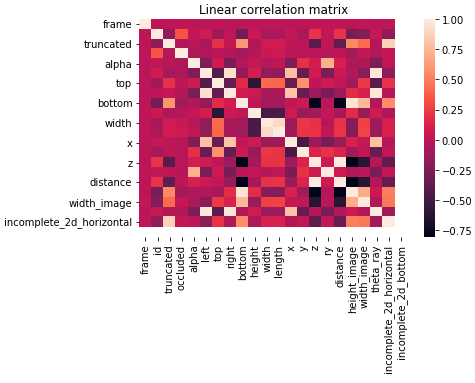
\includegraphics[width=0.6\textwidth]{Book/figures/6_approx_distancia/corr_matrix_kitti.png}
    \caption{Matriz de correlación de las características analizadas.}
    \label{fig:Matriz de correlación de las características analizadas.}
\end{figure}

Dentro de este mismo análisis se estudia de manera muy superficial las características del dataset que tienen una mayor relación con la distancia ya que es necesario obtener con que característica se puede obtener la distancia, tal y como se tratará se realizar en el siguiente capítulo. Para ello se construye una matriz de correlación mediante el uso del coeficiente de correlación de Pearson: $\rho_{X,Y} = \sigma_{X,Y}/(\sigma_X \sigma_Y)$. La Figura \ref{fig:Matriz de correlación de las características analizadas.} muestra dicha matriz de correlación en la que se observa como son: la recta horizontal inferior de la bounding box 2D, el eje Z del centro tridimensional, la altura de la bounding box 2D y la anchura de la bounding box 2D; aquellos parámetros que tienen un índice de correlación mayor con la distancia.

Habiendo obtenido las características más relevantes para la obtención de la distancia a los objetos, se visualiza en un gráfico de dispersión con la relación entre estos y la distancia, para obtener la característica a utilizar en la predicción de la distancia. La Figura \ref{fig:Gráficos de dispersión entre la distancia y las características con más correlación.} muestra todos los gráficos de dispersión, teniendo en el eje de ordenadas la distancia a los objetos y en el eje de abscisas las características estudiadas. En este gráfico se observa como a partir del eje Z del centro tridimensional se puede obtener directamente la distancia, de forma adicional, a partir de la recta horizontal inferior de la bounding box 2D y la altura de la bounding box 2D se puede obtener también la distancia pero con algo más de error, por último, con la la anchura de la bounding box 2D no se puede obtener la distancia de forma sencilla sin asumir un error muy grande.

\begin{figure}[H]
    \centering
    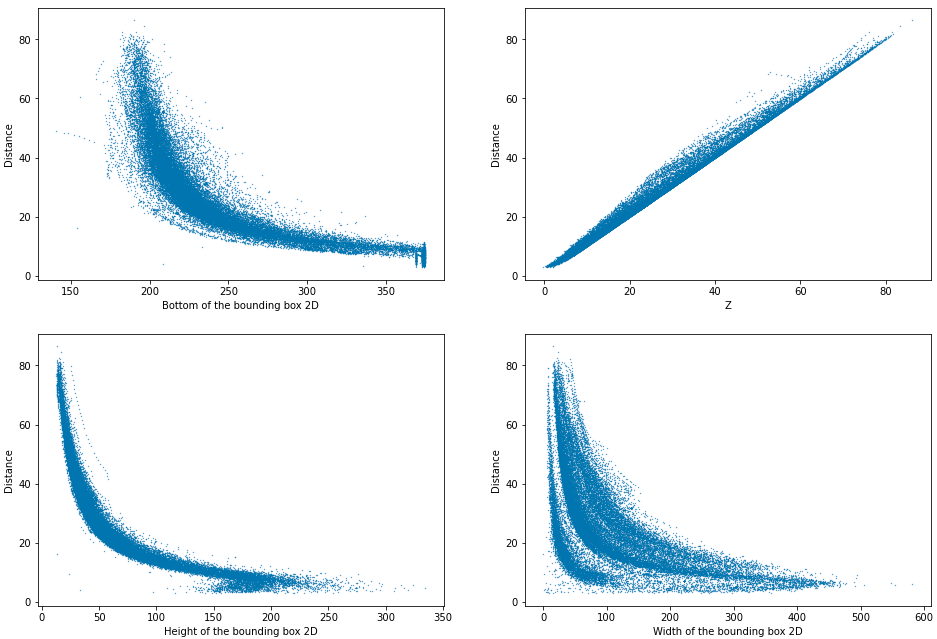
\includegraphics[width=0.9\textwidth]{Book/figures/6_approx_distancia/metrics_to_get_distance_kitti.png}
    \caption{Gráficos de dispersión entre la distancia y las características con más correlación.}
    \label{fig:Gráficos de dispersión entre la distancia y las características con más correlación.}
\end{figure}

Debido a que el eje Z del centro tridimensional de los objetos no se conoce de antemano, se decide utilizar para obtener la distancia a los objetos, la altura de la bounding box 2D. Esto es así, ya que de forma comparativa con la recta horizontal inferior de la bounding box 2D, se tiene una menor dispersión, además de estar asumiendo con este parámetro que el vehículo se encuentra siempre en una carretera sin pendientes, ya que el dataset de KITTI no contiene ninguna situación con esta característica.

\section{Modelo basado en la altura del objeto 2D}
\label{sec:Modelo basado en la altura del objeto 2D}

Habiendo elegido la característica que permite de mejor manera la obtención de la distancia, se trata de obtener una función que ajuste la distancia tras la obtención de la bounding box 2D de cada objeto. Este ajuste de la función no se realiza sobre la salida del modelo \ac{YOLO}v5, sino que parte del ground-truth de KITTI para su ajuste con los datos de entrenamiento, y se comprueba la efectividad de dicho ajuste sobre los datos de validación.

La métrica definida para la evaluación de todos los modelos de aproximación de la distancia es el \ac{MSE}, el cual se define por la siguiente función: $\textit{MSE} = \frac{1}{n} \sum_{i=1}^{n} (Y_i - \hat{Y}_i)^2$. Esta métrica es elegida ya que elimina los errores positivos y negativos, además de castigar de forma cuadrática los errores más grandes, lo cual permitirá discernir de mejor manera el modelo que más se ajusta.

En cuanto al modelo de ajuste, se decide optar por un sencillo modelo de regresión (no lineal) ya que permite su creación de forma sencilla además de permitir una ejecución de forma inmediata sin añadir carga de trabajo a todo el pipeline de detección 3D. Para realizar el ajuste de la función a utilizar que tenga de entrada la altura de la bounding box 2D y como salida la distancia al objeto, se utiliza la librería Scikit-learn. Mediante el uso de dicha librería en Python, se definen múltiples funciones polinómicas y logarítmicas para que mediante un ajuste por mínimos cuadrados se obtengan los valores que compongan las diferentes funciones.

En la Figura \ref{fig:Ajuste de diversas funciones para la obtención de la distancia.} se observan 6 de las funciones que se han probado para ajustar la obtención de la distancia. En esta imagen se observa como las funciones polinómicas no son capaces de ajustarse de forma correcta a las características de la curva definida por la relación entre las características analizadas. Por otra parte, las funciones funciones logarítmicas utilizadas son aquellas que mejor se ajustan, siendo la siguiente función aquella que mejor se ajusta: $y = a \log{x}^b + c; a = 668,12; b = -2; c = -17,39$.

\begin{figure}[H]
    \centering
    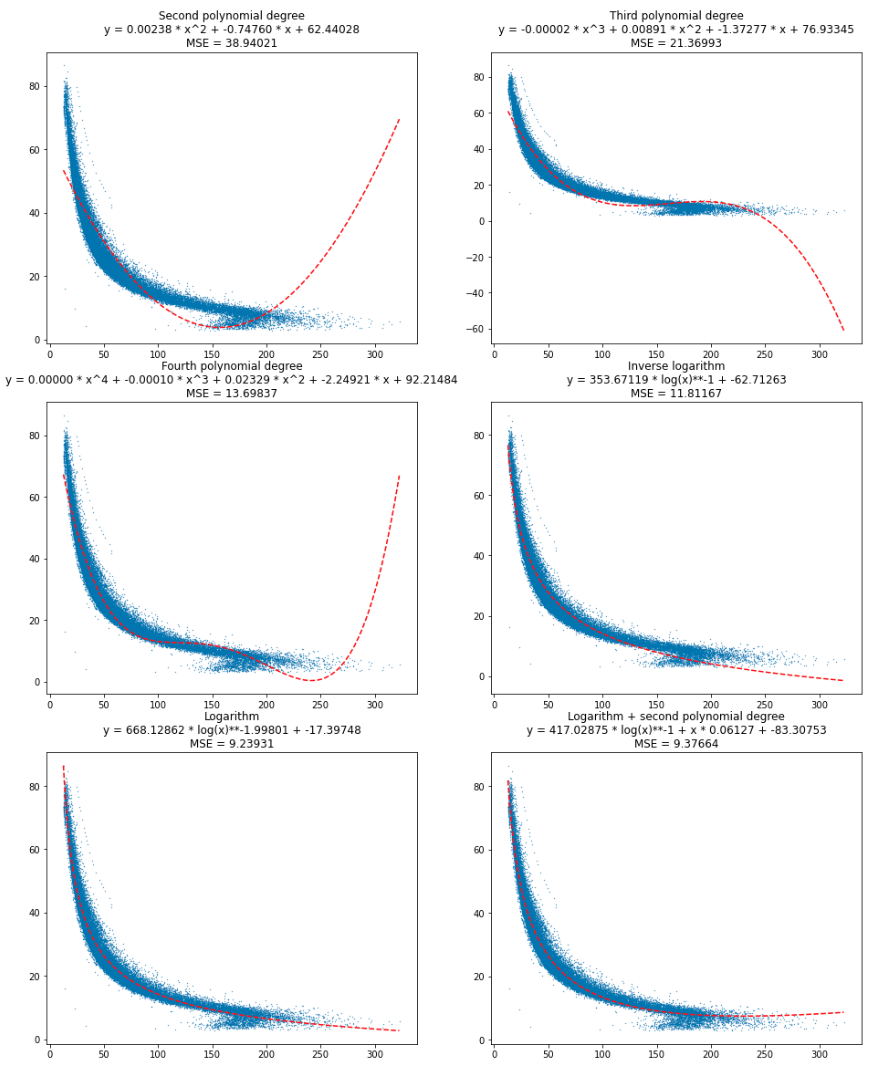
\includegraphics[width=0.7\textwidth]{Book/figures/6_approx_distancia/distance_regression_1_kitti1.png}
    \caption{Ajuste de diversas funciones para la obtención de la distancia.}
    \label{fig:Ajuste de diversas funciones para la obtención de la distancia.}
\end{figure}

Habiendo observado en el capítulo anterior que cada una de las clases de objetos utilizados tiene unas dimensiones diferentes, se plantea la creación de una función por cada una de las tres clases a detectar. Para ello se utilizará la función logarítmica previamente obtenida que se ajusta de mejor manera a los datos.

Tras la obtención de las parámetros de esta función logarítmica se obtienen las diferentes curvas que ajustan la relación entre la distancia y altura de la bounding box 2D para cada una de las clases. Esto se realiza de esta manera debido a que la altura media de cada una de las clases es diferente, por lo que el ajuste al realizarse de forma individual por cada clase de puede mejorar la precisión de las predicciones de la distancia a cada objeto. En la Figura \ref{fig:Ajuste de una función logarítmica por cada clase.} se observa como en las clases peatón y ciclista la métrica de \ac{MSE} se reduce, mientras que en la clase coche se aumenta. Esto es debido a que como se vio previamente, el 80\% de los objetos de los objetos son coches, por lo que se les puede encontrar en muchas más situaciones complejas.

\begin{figure}[H]
    \centering
    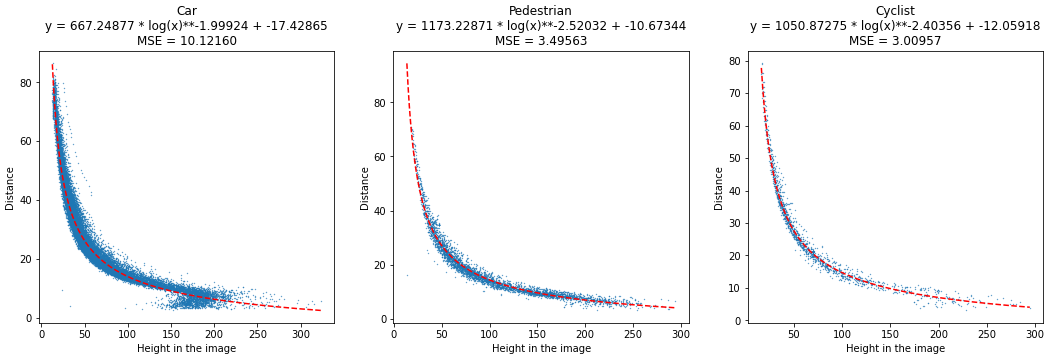
\includegraphics[width=1\textwidth]{Book/figures/6_approx_distancia/regression_classes_kitti1.png}
    \caption{Ajuste de una función logarítmica por cada clase.}
    \label{fig:Ajuste de una función logarítmica por cada clase.}
\end{figure}

Analizando el resto de características con las que se puede trabajar para obtener una aproximación de la distancia más precisa, se encuentra que la completitud horizontal de las bounding boxes 2D de los objetos, definida como aquellas bounding boxes que se encuentran en el límite izquierdo o derecho de la imagen, pueden aportar información al modelo, ya que aquellas bounding boxes que cumplen esta propiedad, no se conoce de forma correcta la altura de su bounding box 2D al no encontrarse el objeto al completo dentro del \ac{FoV} de la cámara. Se ha observado de forma adicional, como el análisis únicamente de la componente horizontal de la bounding box 2D aporta más información que el uso de la componente vertical o la combinación de ambas.

En la Figura \ref{fig:Resaltado de las bounding box 2D no completas horizontalmente.} se puede ver de forma resaltada en naranja aquellos objetos que cumplen con el filtro de bounding boxes 2D incompletas horizontalmente. En dichos puntos naranjas se observa una distribución diferente a la encontrada de forma general en el resto del dataset, por lo que se decide incorporar este parámetro al modelo a utilizar. 

\begin{figure}[H]
    \centering
    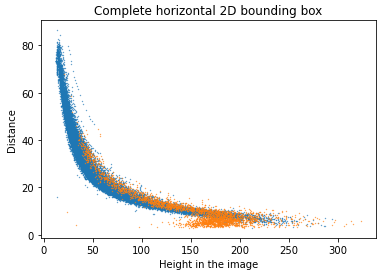
\includegraphics[width=0.5\textwidth]{Book/figures/6_approx_distancia/bb_complete_kitti1.png}
    \caption{Resaltado de las bounding box 2D no completas horizontalmente.}
    \label{fig:Resaltado de las bounding box 2D no completas horizontalmente.}
\end{figure}

Habiendo definido el uso de una nueva característica es necesario definir con que técnica tratarla, en este caso, al observarse en la figura anterior una nueva curva con los datos filtrados según la nueva característica a utilizar se decide ajustar de forma separada dos curvas logarítmicas como se ha hecho previamente. Durante el análisis de esta característica se ha observado que en las clases 'peatón' y 'ciclista' hay muy pocos casos en los que las bounding boxes 2D no se encuentren completas, debido a esto, para evitar un caso de sobreajuste se decide utilizar la clase 'coche' como la única por la que filtrar y ajustar una función en relación a la completitud de la bounding box 2D.

En la Figura \ref{fig:Ajuste de la distancia a los coches en función de la completitud de la bounding box 2D.} se muestra el ajuste de las dos curvas en función de la nueva característica a introducir en el modelo sobre la clase 'coche', de esta manera se consigue que las vehículos que cumplen esta característica tengan una distancia aproximada más precisa.

\begin{figure}[H]
	\begin{minipage}{0.45\textwidth}
		\centering
		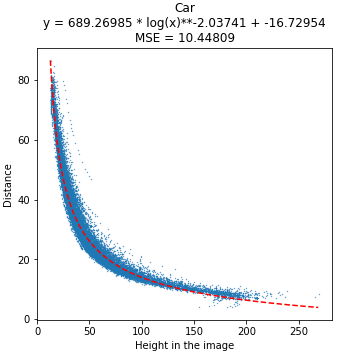
\includegraphics[width=0.87\linewidth]{Book/figures/6_approx_distancia/car_bb_complete_kitti1.png}
	\end{minipage}\hfill
	\begin{minipage}{0.45\textwidth}
		\centering
		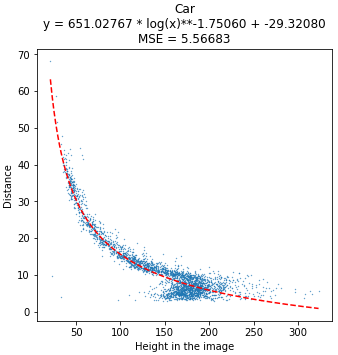
\includegraphics[width=0.9\linewidth]{Book/figures/6_approx_distancia/car_bb_incomplete_kitti1.png}
	\end{minipage}
	\caption{Ajuste de la distancia a los coches en función de la completitud de la bounding box 2D.}
	\label{fig:Ajuste de la distancia a los coches en función de la completitud de la bounding box 2D.}
\end{figure}

Como forma de estudiar los resultados obtenidos del sistema de aproximación de la distancia, se decide utilizar un método de evaluación común entre todos los modelos que sean diseñados, para ello se va a basar en el método de evaluación de KITTI y la métrica definida hasta ahora como es el \ac{MSE}.

Dentro de la evaluación de KITTI se define el concepto de dificultad entre los diferentes objetos a detectar, para los cuales se usa la altura de los objetos sobre la imagen, la oclusión (valor en función de la visibilidad del objeto que puede variar de 0 a 3) y el porcentaje de truncamiento de los objetos sobre el \ac{FoV} de la cámara. las diferentes dificultades con las que se trabaja son:
\begin{itemize}
    \item 'Fácil': son aquellos objetos con una altura en la imagen mayor de 40 píxeles, un valor de oclusión de 0 y un truncamiento máximo del 15\%.
    \item 'Moderado': son aquellos objetos con una altura en la imagen mayor de 25 píxeles, un valor de oclusión máximo de 1 y un truncamiento máximo del 30\%.
    \item Difícil: son aquellos objetos con una altura en la imagen mayor de 25 píxeles, un valor de oclusión máximo de 2 y un truncamiento máximo del 30\%.
\end{itemize}
El resto de los objetos que no se incluyen en ninguna de las diferentes categorías no se estudian, aunque más adelante se verá un caso en el que aquellos objetos sin dificultad han sido de relevancia.

Tras la definición del método de evaluación que se compone de las dificultades, la métrica (\ac{MSE}) y el estudio a nivel de clase, se calculan las métricas obtenidas en este primer método de aproximación de la distancia basado en la altura de las bounding boxes 2D.

\begin{table}[H]
\centering
\begin{tabular}{|c|c|c|c|}
\hline
\textbf{Benchmark (MSE)} & \textbf{Fácil} & \textbf{Moderado} & \textbf{Difícil} \\ \hline \hline
Coche (distancia)        & 8,724          & 9,115             & 9,127            \\ \hline
Peatón (distancia)       & 4,643          & 5,902             & 5,645            \\ \hline
Ciclista (distancia)     & 3,822          & 4,444             & 4,469            \\ \hline
\end{tabular}
\caption{Evaluación sobre KITTI del modelo de aproximación de distancia basado en regresión.}
\label{tab:Evaluación sobre KITTI del modelo de aproximación de distancia basado en regresión.}
\end{table}

La Tabla \ref{tab:Evaluación sobre KITTI del modelo de aproximación de distancia basado en regresión.} muestra unos resultados bastante buenos de este modelo de aproximación de distancia, el cual solo requiere de una imagen de las bounding boxes 2D que pueden ser obtenidas por un modelo como YOLOv5. Tras este primer modelo se estudiaran otros que traten de mejorar estos primeros resultados que son claramente bastante buenos pero mejorables.

\section{Modelo basado en la proyección de la nube de puntos}
\label{sec:Modelo basado en la proyección de la nube de puntos}

Habiendo obtenido un modelo de aproximación de la distancia basado únicamente en la cámara del vehículo, se ha decido utilizar también en un modelo diferente la nube de puntos proporcionada por el \ac{LiDAR}. Mientras que la cámara no tiene ningún método directo con el que calcular la distancia a los objetos, con el \ac{LiDAR} se puede calcular la distancia a cualquier punto de la nube de puntos obtenida por dicho sensor de forma precisa.

Partiendo del uso de bounding boxes 2D que pueden ser obtenidas por el modelo YOLOv5 presentado en la Sección \ref{sec:Entrenamiento y evaluación de YOLOv5}, se decide trabajar de forma conjunta con dichas detecciones 2D junto con el \ac{LiDAR} para analizar los puntos que se encuentran dentro de las bounding boxes. Mientras que esto parece una tarea sencilla es necesario estudiar las transformaciones de mundo a cámara de una lente como se observa en la Figura \ref{fig:Transformaciones mundo a cámara.} para poder pasar del sistema de coordenadas del LiDAR a la cámara.

\begin{figure}[H]
    \centering
    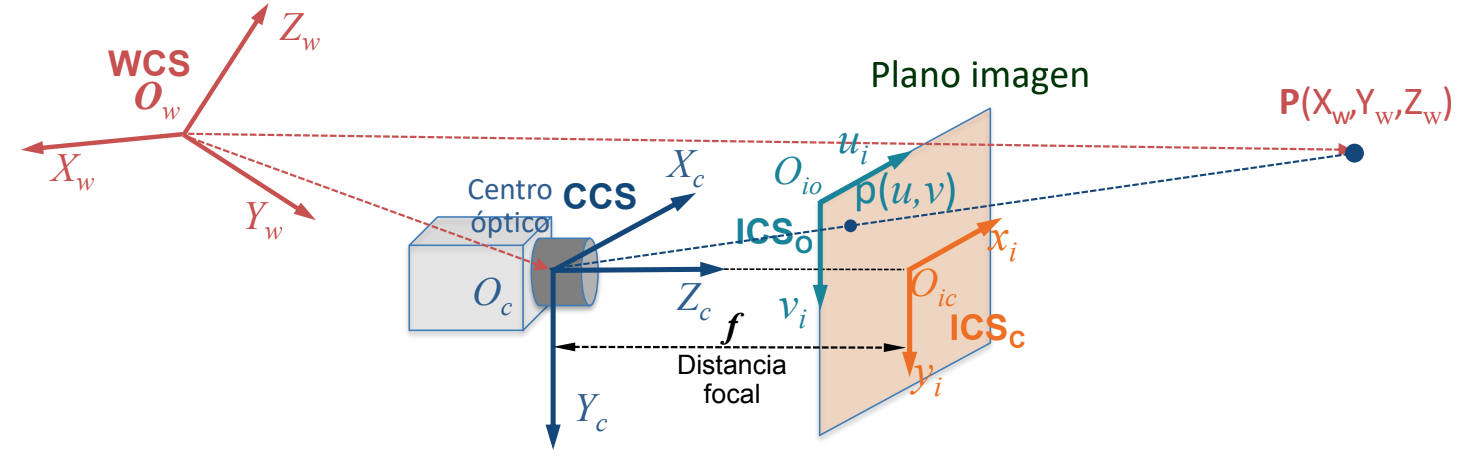
\includegraphics[width=0.7\textwidth]{Book/figures/6_approx_distancia/funcionamiento_camara.png}
    \caption{Transformaciones mundo a cámara.}
    \label{fig:Transformaciones mundo a cámara.}
\end{figure}

Tras el estudio de las transformaciones necesarias para obtener la nube de puntos sobre las imágenes obtenidas por la cámara se estudiaran los puntos para tratar de obtener un modelo que mejore al modelo anterior basado únicamente en la cámara. Para ello se plantea utilizar la mediana de la distancia de los puntos dentro de cada objeto y posteriormente se aplicará un pequeño modelo que obtenga la distancia al centro de cada objeto.

\subsection{Sistema de proyección de la nube de puntos a la cámara}
\label{sec:Sistema de proyección de la nube de puntos a la cámara}

Las nubes de puntos dadas en el dataset de KITTI siguen un formato típico en el cual a partir de un archivo binario se guarda la información de cada punto definida por los parámetros: 'x', 'y', 'z' y 'intensidad'; los cuales tienen un formato de números decimales de 32 bits. Dentro de las transformaciones geométricas a realizar solo es necesario utilizar las coordenadas tridimensionales de cada punto para realizar la traslación, rotación y cambio en el sistema de coordenadas de la nube de puntos. Para la comprensión de las operaciones realizadas en esta transformación es necesario comprender primero el funcionamiento de las proyecciones mundo a cámara las cuales son utilizadas en dicha proyección.

Como primer paso dentro de este proceso de la proyección de la nube de puntos a la cámara, es necesario el sistema de coordenadas a utilizar. En este caso se ha definido un sistema de coordenadas homogéneas para simplificar ciertos pasos más adelante, por lo que es necesario transformar el sistema de coordenadas cartesiano a este sistema de la manera definida por las siguientes fórmulas.

\begin{center}
$(x, y, z) \rightarrow (x', y', z', w)$\\[10pt]
$(x, y, z) = (x'/w, y'/w, z'/w)$
\end{center}

Tras la transformación al sistema de coordenadas homogéneo, se trata de cambiar el sistema de coordenadas actual al dado por la cámara con la que se trabaja, para ello es necesario realizar una traslación al sistema de coordenadas de la cámara y tras esto una rotación de los ejes para que concuerden con el sistema de coordenadas de la cámara. Al trabajar con las coordenadas homogéneas, la traslación del eje de coordenadas no es más que una multiplicación de matrices como se puede observa en la siguiente fórmula.

\begin{center}
$
\begin{bmatrix} wX_c \\ wY_c \\ wZ_c \\ w \end{bmatrix}
=
\begin{bmatrix}
1 & 0 & 0 & T_X \\
0 & 1 & 0 & T_Y \\
0 & 0 & 1 & T_Z \\
0 & 0 & 0 & 1 \\
\end{bmatrix}
\begin{bmatrix} X_w \\ Y_w \\ Z_w \\ 1 \end{bmatrix}
$
\end{center}

En cuanto a la rotación del sistema de coordenadas, es necesario entender que la rotación se realiza en los tres diferentes ejes, por lo que hay que utilizar una matriz de rotación por cada uno de los ejes, lo cual es una multiplicación de cuatro matrices.

\begin{center}
$R = R_X(\alpha) R_Y(\beta) R_Z(\gamma)$
\end{center}

\begin{center}
$
\begin{bmatrix} wX_c \\ wY_c \\ wZ_c \\ w \end{bmatrix}
=
\begin{bmatrix}
1 & 0 & 0 & 0 \\
0 & \cos \alpha & -\sin \alpha & 0 \\
0 & \sin \alpha & \cos \alpha & 0 \\
0 & 0 & 0 & 1 \\
\end{bmatrix}
\begin{bmatrix}
\cos \beta & 0 & \sin \beta & 0 \\
0 & 1 & 0 & 0 \\
- \sin \beta & 0 & \cos \beta & 0 \\
0 & 0 & 0 & 1 \\
\end{bmatrix}
\begin{bmatrix}
\cos \gamma & - \sin \gamma & 0 & 0 \\
\sin \gamma & \cos \gamma & 0 & 0 \\
0 & 0 & 1 & 0 \\
0 & 0 & 0 & 1 \\
\end{bmatrix}
\begin{bmatrix} X_w \\ Y_w \\ Z_w \\ 1 \end{bmatrix}
$
\end{center}

Otra opción es multiplicar desde un principio la matriz de traslación y las tres matrices de rotación que son fijas si no se mueve ninguno de los dos sistemas de coordenadas con los que se trabaja, y trabajar con una única matriz para reducir la complejidad de la fórmula además de reducir el numero de operación a realizar por un ordenador. Esta matriz es denominada la matriz de parámetros extrínsecos.

\begin{center}
$
\begin{bmatrix} wX_c \\ wY_c \\ wZ_c \\ w \end{bmatrix}
=
\begin{bmatrix}
\cos \gamma \cos \beta & - \sin \gamma \cos \beta & \sin \beta & T_X \\
\cos \gamma \sin \alpha \sin \beta + \sin \gamma \cos \alpha & \cos \gamma \cos \alpha - \sin \gamma \sin \alpha \sin \beta & - \sin \alpha \cos \beta & T_Y \\
\sin \gamma \sin \alpha - \cos \gamma \cos \alpha \sin \beta & \sin \gamma \cos \alpha \sin \beta + \cos \gamma \sin \alpha & \cos \alpha \cos \beta & T_Z \\
0 & 0 & 0 & 1 \\
\end{bmatrix}
\begin{bmatrix} X_w \\ Y_w \\ Z_w \\ 1 \end{bmatrix}
$
$
M_{ext}
=
\begin{bmatrix}
r_{11} & r_{12} & r_{13} & t_X \\
r_{21} & r_{22} & r_{23} & t_Y \\
r_{31} & r_{32} & r_{33} & t_Z \\
\end{bmatrix}
$
\end{center}

Tras este cambio del sistema de coordenadas al mismo con el que trabaja la cámara, es necesario pasar a nivel de píxel para comprender como cada punto del entorno tridimensional pasa a encontrarse dentro de las imágenes producidas por una cámara. Dentro de este proceso, es necesario comprender los parámetros intrínsecos que afectan en el paso del mundo real tridimensional al mundo bidimensional de las imágenes.

El primer parámetro a tener en cuenta es la distancia focal ($f$), la cual es la distancia entre el centro óptico de la lente y el foco de la cámara. Este parámetro es utilizado para pasar al sistema de coordenadas bidimensionales de la cámara pero en el sistema métrico.

\begin{center}
$
\begin{bmatrix} wx \\ wy \\ w \end{bmatrix}
=
\begin{bmatrix}
f & 0 & 0 & 0 \\
0 & f & 0 & 0 \\
0 & 0 & 1 & 0 \\
\end{bmatrix}
\begin{bmatrix} X_c \\ Y_c \\ Z_c \\ 1 \end{bmatrix}
$
\end{center}

Para obtener los puntos proyectados en los píxeles de las imágenes, se pasa al sistema de coordenadas pixélicas, definido por el tamaño en píxeles ($dx$, $dy$) y el desplazamiento al origen de las imágenes ($u_0$, $v_0$).

\begin{center}
$
\begin{bmatrix} wu \\ wv \\ w \end{bmatrix}
=
\begin{bmatrix}
1/dx & 0 & u_0 \\
0 & 1/dy & v_0 \\
0 & 0 & 1 \\
\end{bmatrix}
\begin{bmatrix} wx \\ wy \\ w \end{bmatrix}
$
\end{center}

De la misma manera que se construye la matriz de parámetros extrínsecos, se multiplican las dos últimas matrices relacionadas con los parámetros internos de la cámara, para construir una matriz de parámetros intrínsecos y simplificar el tratamiento de una cámara dada, ya que estos parámetros son fijos a una cámara concreta y no se modifican.

\begin{center}
$
M_{int}
=
\begin{bmatrix}
1/dx & 0 & u_0 \\
0 & 1/dy & v_0 \\
0 & 0 & 1 \\
\end{bmatrix}
\begin{bmatrix}
f & 0 & 0 \\
0 & f & 0 \\
0 & 0 & 1 \\
\end{bmatrix}
=
\begin{bmatrix}
f/dx & 0 & u_0 \\
0 & f/dy & v_0 \\
0 & 0 & 1 \\
\end{bmatrix}
$
\end{center}

De forma sencilla, se puede obtener la transformación de puntos tridimensionales del entorno a la cámara a partir de las matrices de parámetros extrínsecos e intrínsecos con unas simples multiplicaciones.

\begin{center}
$
\begin{bmatrix} wu \\ wv \\ w \end{bmatrix}
=
M_{int} M_{ext}
\begin{bmatrix} X_w \\ Y_w \\ Z_w \\ 1 \end{bmatrix}
$
\end{center}

Hasta ahora se ha explicado de forma teórica como funcionan las transformaciones necesarias para trabajar con cámara y comprender su tratamiento, pero en este apartado se explicará su uso práctico a partir de las matrices de calibración dadas en el dataset de KITTI y que han tenido que ser utilizadas para realizar todas las transformaciones geométricas necesarias en este apartado para la proyección de la nube de puntos además de su uso en la creación de 'troncos geométricos' como se verá en el Capítulo \ref{cha:Obtención de la región de interés}.

En este caso de uso concreto que se quiere obtener, es necesario trabajar con tres matrices diferentes con las que se logrará pasar del sistema de coordenadas de las nubes de puntos del \ac{LiDAR} a los píxeles de las imágenes dadas por el dataset de KITTI. Estas tres matrices son (según los nombres de dados por KITTI) las siguientes:

\begin{itemize}
    \item $P2$: Esta matriz se compone de la matriz intrínseca de la cámara 2, la cual es la cámara de la cual se van a utilizar las imágenes al ser aquella según se dan las detección 2D además de estar en color y no en escala de grises, además de la traslación respecto de la cámara 0 del vehículo utilizado para la creación de dataset.
    \item $R0\_rect$: Las lentes de la una cámara es muy difícil que sean perfectas, por lo que se suele aplicar una matriz de rectificación que tiene como función eliminar las imperfecciones en las imágenes como pueden ser las distorsiones de barril y de cojín. Esta matriz trata de solucionar estos problemas de las imágenes obtenidas por el sensor de la misma manera que se realiza con cual otro tipo de cámara (a menos que se trabaja con una lente con un error mínimo).
    \begin{center}
    $
    \textit{R0\_rect} = R_{Xr}(\alpha_r) R_{Yr}(\beta_r) R_{Zr}(\gamma_r) 
    \begin{bmatrix} 1&0&0&T_{Xr} \\ 0&1&0&T_{Yr} \\ 0&0&1&T_{Zr} \\ 0&0&0&1 \end{bmatrix}
    $
    \end{center}
    \item $Tr\_velo\_to\_cam$: Esta matriz se compone de la matriz de traslación del sistema de coordenadas del \ac{LiDAR} al sistema de coordenadas de la cámara 0 y de su correspondiente matriz de rotación.
    \begin{center}
    $
    \textit{Tr\_velo\_to\_cam} = R_{X\textit{v2c}}(\alpha_\textit{v2c}) R_{Yr}(\beta_\textit{v2c}) R_{Z\textit{v2c}}(\gamma_\textit{v2c}) 
    \begin{bmatrix} 1&0&0&T_{X\textit{v2c}} \\ 0&1&0&T_{Y\textit{v2c}} \\ 0&0&1&T_{Z\textit{v2c}} \\ 0&0&0&1 \end{bmatrix}
    $
    \end{center}
\end{itemize}

La conversión de la nube de puntos a las imágenes del dataset es muy sencilla si se conoce el funcionamiento de todas estas matriz, ya que simplemente es necesario multiplicar la nube de puntos completa por otras tres matrices diferentes como son: $P2$, $R0\_rect$ y $Tr\_velo\_to\_cam$.

\begin{center}
$
\textit{cam} = \textit{P2} * \textit{R0\_rect} * \textit{Tr\_velo\_to\_cam} * \textit{pcl}
$
\end{center}

\subsection{Aproximación de la distancia a partir de la nube de puntos}
\label{sec:Aproximación de la distancia a partir de la nube de puntos}

Partiendo del hecho que se conoce la manera de proyectar las nubes de puntos sobre las imágenes dadas, se abre una oportunidad para estudiar la distancia a los objetos a partir de dicha nube de puntos y las detecciones 2D que se pueden obtener de los objetos del entorno. La Figura \ref{fig:Proyección de la nube de puntos sobre la cámara.} muestra la manera en la que se proyecta la nube de puntos sobre la imagen que se da de entrada visualizando con colores la distancia del objeto con el colisiona cada láser del \ac{LiDAR} representado por un punto en la imagen.

\begin{figure}[H]
    \centering
    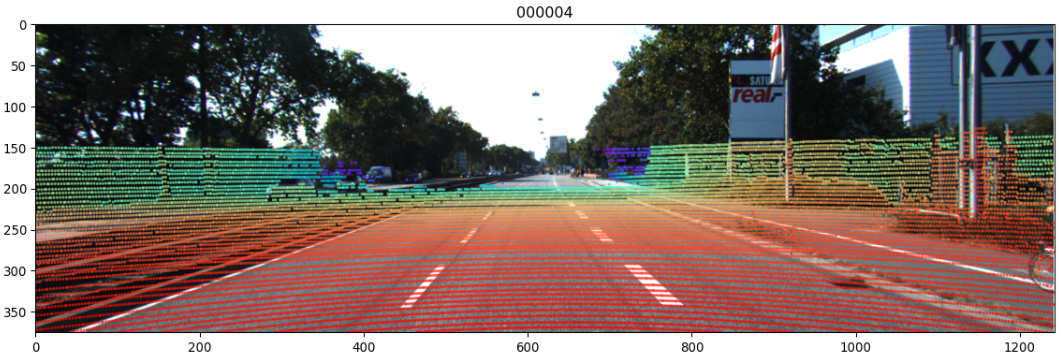
\includegraphics[width=0.8\textwidth]{Book/figures/6_approx_distancia/pcl_projection_kitti2.png}
    \caption{Proyección de la nube de puntos sobre la cámara.}
    \label{fig:Proyección de la nube de puntos sobre la cámara.}
\end{figure}

Mientras que el proceso de segmentación semántica puede ser muy útil y preciso para aproximar la distancia a los objetos del entorno, ya que permite utilizar solo los puntos que se encuentran en los vehículos y no aquellos puntos que no incidan en el objeto de interés, pero se deciden utilizar detecciones 2D ya que con modelos con esta tarea se pueden obtener de manera más rápida dichas detecciones además de diferenciar objetos diferentes si se encuentran muy cerca (cosa que no se puede con un modelo de segmentación semántica). En este análisis por tanto se usará el ground-truth 2D de las imágenes para la realización de las aproximaciones de la distancia a los objetos del entorno.

A partir de la sección de la nube de puntos que se encuentra dentro de las detecciones 2D, se podría calcular la distancia a cada uno de los puntos proyectados y asumir la media de la distancia a todos esos puntos como la distancia a cada objeto del entorno, pero esta distancia se vería afectada por los puntos que se encuentren dentro de las detecciones 2D y que no colisionan con los objetos detectados. Por ello, para reducir los outliers o puntos que no se encuentren en los objetos detectados, se aplica la mediana de la distancia a cada uno de los puntos que se encuentran dentro de las bounding boxes 2D.

\begin{figure}[H]
    \centering
    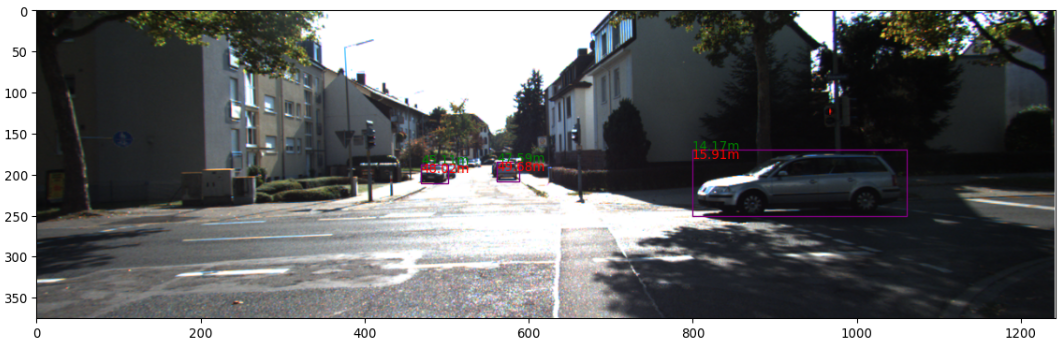
\includegraphics[width=0.8\textwidth]{Book/figures/6_approx_distancia/pcl_projection_distance_kitti2.png}
    \caption{Aproximación de la distancia mediante la nube de puntos.}
    \label{fig:Aproximación de la distancia mediante la nube de puntos.}
\end{figure}

En la Figura \ref{fig:Aproximación de la distancia mediante la nube de puntos.} se puede ver en cada uno de los vehículos de la escena junto con su bounding box 2D, la distancia real en rojo y la distancia obtenida a partir de la nube de puntos en tal como se ha explicado en verde. Si se observa más de cerca, se puede apreciar como todas las distancias reales son superiores a aquellas que han sido detectadas por este método, esto es debido a que a partir de los puntos utilizados se obtiene la distancia al chasis del vehículo y no al centro del vehículo tal y como se estudia en el ground-truth. Esto problema se presentará más en profundidad en la próxima sección.

\begin{table}[H]
\centering
\begin{tabular}{|c|c|c|c|c|}
\hline
\textbf{Benchmark (MSE)} & \textbf{Fácil} & \textbf{Moderado} & \textbf{Difícil} & \textbf{Todo}\\ \hline \hline
Coche (distancia)        & 4,084          & 15,759             & 29,198   &42,346         \\ \hline
Peatón (distancia)       & 3,355          & 6,223             & 13,516    &13,500         \\ \hline
Ciclista (distancia)     & 7,134          & 11,968             & 12,902   &12,857        \\ \hline
\end{tabular}
\caption{Evaluación del modelo de aproximación de distancia basado en nube de puntos.}
\label{fig:Evaluación sobre KITTI del primer modelo de aproximación de distancia basado en nube de puntos.}
\end{table}

A partir de este primer modelo de aproximación de la distancia basado en la nube de puntos se evalúa de la misma manera que con el método basado en la altura de las bounding boxes 2D para así poder comparar sus resultados. La Tabla \ref{fig:Evaluación sobre KITTI del primer modelo de aproximación de distancia basado en nube de puntos.} muestra los resultados de dicha evaluación, en los cuales se puede observar como este método empeora bastante la aproximación de la distancia tal y como se tenía antes. Esto es un problema ya que el sensor \ac{LiDAR} es capaz de dar la posición 3D de cada uno de los puntos de manera muy precisa, por lo que hay factores que no se están teniendo en cuenta como objetos que se solapan a bounding boxes 2D con gran parte de sus píxeles que no pertenecen a los objetos de interés.

\begin{figure}[H]
    \centering
    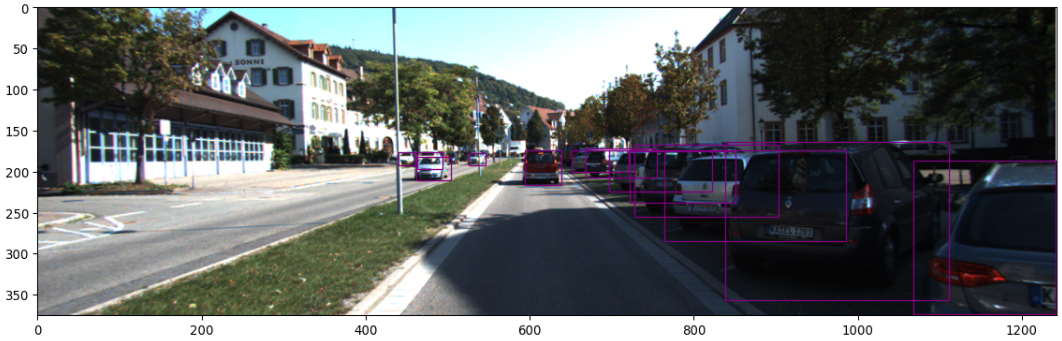
\includegraphics[width=0.8\textwidth]{Book/figures/6_approx_distancia/bb2d_kitti2.png}
    \caption{Caso de dificultad para obtener la distancia a partir de la nube de puntos.}
    \label{fig:Caso de dificultad para obtener la distancia a partir de la nube de puntos.}
\end{figure}

Para ejemplificar estos casos en los que las bounding boxes 2D de una imagen se solapan, se presenta la Figura \ref{fig:Caso de dificultad para obtener la distancia a partir de la nube de puntos.} en la que se tienen multitud de vehículos aparcados de forma muy cercana y la gran mayoría de ellos se están solapando al igual de las bounding boxes del dataset de KITTI. Además de este tipo de de oclusiones, hay que tener en cuenta las posibles oclusiones con otros objetos del entorno que no sean detectados, como: farolas, papeleras o árboles; además de los objetos truncados que se encuentren en los bordes de la imagen.

Como solución parcial a este problema que se observa en la imagen anterior, el cual afecta principalmente a los coches, se planea el uso del modelo de aproximación de la distancia anterior (basado en la altura de las bounding boxes 2D) para calcular que objetos se encuentran delante y cuales detrás en la imagen con la que se trabaja. De esta manera, los puntos que se encuentren en las intersecciones de las bounding boxes de los objetos de la parte frontal, solo serán utilizados para la aproximación de la distancia del objeto que se encuentre más cerca a la cámara. Gracias a esto, se espera que los puntos que interceden en varias bounding boxes, no perjudiquen al resto de objetos en los que no inciden dichos puntos del \ac{LiDAR}.

\begin{table}[H]
\centering
\begin{tabular}{|c|c|c|c|c|}
\hline
\textbf{Benchmark (MSE)} & \textbf{Fácil} & \textbf{Moderado} & \textbf{Difícil} & \textbf{Todo}\\ \hline \hline
Coche (distancia)        & 5,143          & 14,861             & 22,961       &29,971     \\ \hline
Peatón (distancia)       & 5,557          & 13,780             & 18,319       &18,032     \\ \hline
Ciclista (distancia)     & 7,107          & 19,733             & 30,106       &25,937  \\ \hline
\end{tabular}
\caption{Evaluación del modelo de aproximación de distancia sin intersecciones en las bounding boxes.}
\label{fig:Evaluación del modelo de aproximación de distancia sin intersecciones en las bounding boxes.}
\end{table}

Los resultados que se pueden ver en la Tabla \ref{fig:Evaluación del modelo de aproximación de distancia sin intersecciones en las bounding boxes.} no son muy prometedores, ya que se mejora la precisión en la aproximación de la distancia en los coches, pero empeora en los peatones y ciclistas. Aún obteniendo resultados peores en dos de las clases a detectar, se decide seguir con este método, debido a que los coches son la clase más difícil para aproximar la distancia, como se vio en la Tabla \ref{tab:Evaluación sobre KITTI del modelo de aproximación de distancia basado en regresión.}, además de la reducción del error máximo de un tipo de objeto con el método anterior de 42,346; en la clase 'coche' a 29,971; en la misma clase, lo cual será un factor muy importe en la construcción del modelo de detección 3D como se verá en la Sección \ref{sec:Creación del modelo Frustum PointPillars}.

\subsection{Modelo de rectificación de la distancia}
\label{sec:Modelo de rectificación de la distancia}

Uno de los problemas de este método de aproximación de la distancia basado en las nubes de puntos es el uso directo de los puntos para obtener la distancia al centro del vehículo, ya que estos surgen de la reflexión de los láseres del \ac{LiDAR} con la primera zona en la que inciden, la cual no es nunca el centro del objeto. Por ello, se ha decidido crear un segundo método para pasar de la distancia a región más cercana de los objetos, a la distancia al centro tridimensional de cada objeto.

\begin{figure}[H]
	\begin{minipage}{0.32\textwidth}
		\centering
		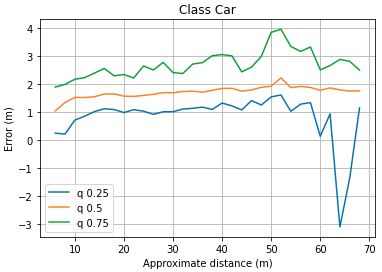
\includegraphics[width=1\linewidth]{Book/figures/6_approx_distancia/error_projection_car_kitti3.png}
	\end{minipage}\hfill
	\begin{minipage}{0.32\textwidth}
		\centering
		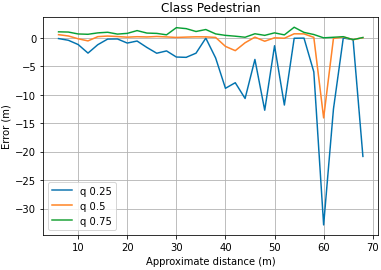
\includegraphics[width=1\linewidth]{Book/figures/6_approx_distancia/error_projection_pedestrian_kitti3.png}
	\end{minipage}\hfill
	\begin{minipage}{0.32\textwidth}
		\centering
		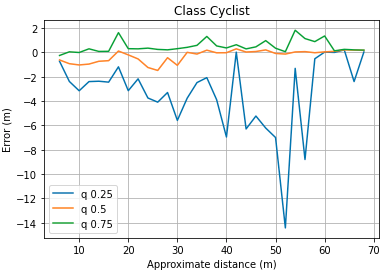
\includegraphics[width=1\linewidth]{Book/figures/6_approx_distancia/error_projection_cyclist_kitti3.png}
	\end{minipage}
	\caption{Error del modelo de de proyección con LiDAR por clase.}
	\label{fig:Error del modelo de de proyección con LiDAR por clase.}
\end{figure}

El primer paso a realizar antes de empezar a crear el segundo modelo para la rectificación de la distancia, es observar los errores obtenidos sobre el dataset, y comprobar que coinciden con el tipo error que se ha razonado. Para ello se analizan los errores de la Figura \ref{fig:Error del modelo de de proyección con LiDAR por clase.}, en los cuales se puede observar como es necesario añadir más distancia en el caso de los coches, mientras que en el caso de los peatones y los ciclistas apenas hace falta modificar nada, si acaso restar cierta parte de la distancia, esto último ocurre debido a que las bounding boxes de los peatones y ciclistas tienen gran cantidad de puntos del \ac{LiDAR} que no inciden en el propio objeto, sino que son parte de objetos tras estos, como: paredes, árboles o asfalto a una mayor distancia. Esto nos indica que estamos en lo cierto, y se puede realizar el modelo de rectificación de la distancia sin temor a que estos errores sean por un sesgo desconocido en la naturaleza de los datos con los que se trabaja.

\begin{figure}[H]
    \centering
    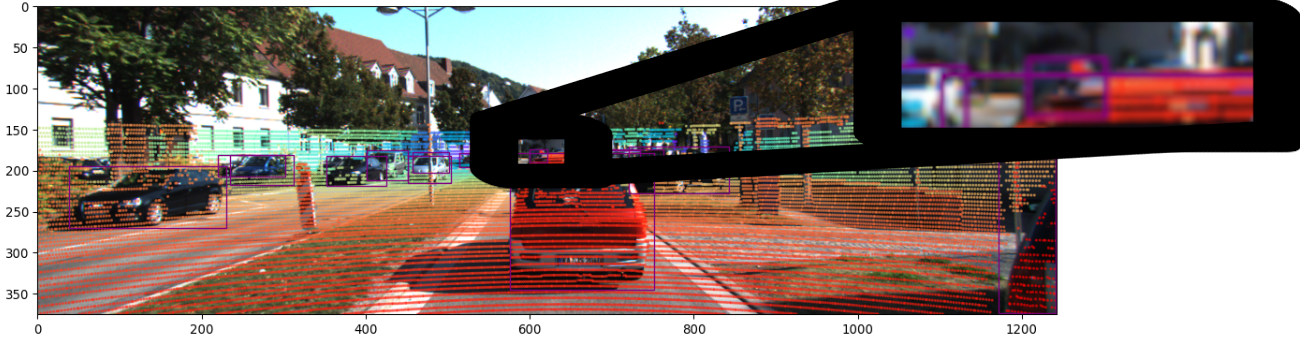
\includegraphics[width=0.8\textwidth]{Book/figures/6_approx_distancia/detail_lidar.png}
    \caption{Caso con gran error en la aproximación de la distancia.}
    \label{fig:Caso con gran error en la aproximación de la distancia.}
\end{figure}

Antes de comenzar a crear dicho modelo de rectificación, se va a observar un caso concreto de aquellos que incrementan el error del modelo previamente creado. La Figura \ref{fig:Caso con gran error en la aproximación de la distancia.} muestra el peor caso en el que un vehículo a más de 50 metros se encuentra con una bounding box 2D y un punto del \ac{LiDAR} con el que se calcula su distancia. El problema de este caso aparece cuando uno observa que dicho punto pertenece a la colisión de un haz láser con la esquina superior izquierda del vehículo que se encuentra en el centro de la imagen, esto es debido a una mala reflexión del láser por lo que en la detección de este por parte del \ac{LiDAR} ha quedado desplazado lo suficiente para que se produzca un error de 50 metros en la distancia inferida debido al funcionamiento del modelo anteriormente presentado. Mientras que este tipo de errores no pueden ser solucionados por este método de aproximación de la distancia, tampoco es un problema que sea muy común, además de que en el pipeline de del sistema completo probablemente no fuera detectado por el modelo YOLOv5 al ser un vehículo tan lejano y ocluido.

Como método elegido en la creación del modelo de rectificación de la distancia, se plantea el uso de funciones matemáticas que definan la magnitud de la rectificación a aplicar a cada uno de los objetos detectados. Durante el proceso de creación de estos modelos, se decide ajustar multitud de funciones matemáticas definidas a mano mediante el uso del descenso por el gradiente para reducir el error cuadrático medio de dicha función sobre los puntos definidos por la distancia inferida y el error producido. Las funciones que mejor se ajustan a los datos con los que se trabajan se muestran en la Figura \ref{fig:Modelo de rectificación de la distancia al centro de los objetos.}, donde de forma adicional se puede observar la distribución de los errores cometidos en función de la distancia como un gráfico de dispersión.

\begin{figure}[H]
	\begin{minipage}{0.32\textwidth}
		\centering
		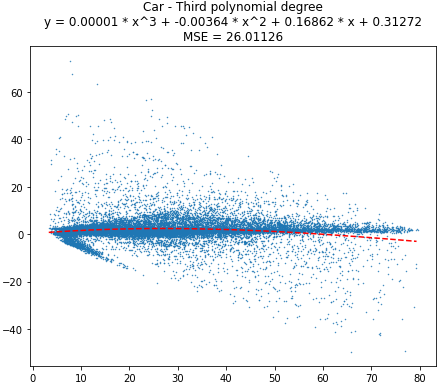
\includegraphics[width=1\linewidth]{Book/figures/6_approx_distancia/rectification_lidar_car.png}
	\end{minipage}\hfill
	\begin{minipage}{0.32\textwidth}
		\centering
		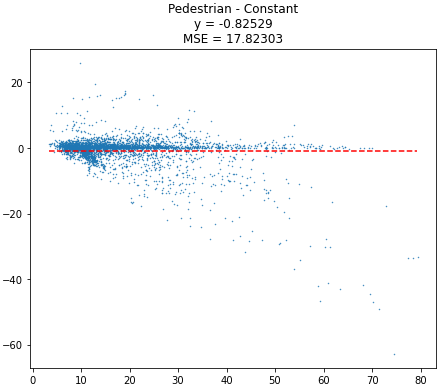
\includegraphics[width=1\linewidth]{Book/figures/6_approx_distancia/rectification_lidar_pedestrian.png}
	\end{minipage}\hfill
	\begin{minipage}{0.32\textwidth}
		\centering
		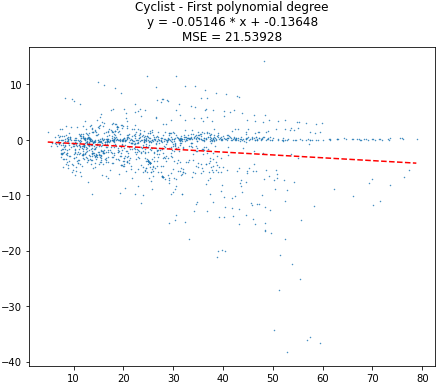
\includegraphics[width=1\linewidth]{Book/figures/6_approx_distancia/rectification_lidar_cyclist.png}
	\end{minipage}
	\caption{Modelo de rectificación de la distancia al centro de los objetos.}
	\label{fig:Modelo de rectificación de la distancia al centro de los objetos.}
\end{figure}

Estas funciones de rectificación definidas logran obtener una precisión mayor en la obtención de la distancia respecto al modelo basado en las nubes de puntos pero sin la rectificación como se puede ver en la Tabla \ref{fig:Evaluación del modelo de aproximación de distancia rectificado.}. Esta mejora se encuentra principalmente en las clases 'coche' y 'ciclista', donde la distancia de la superficie del objeto al centro es mayor, por esto mismo la clase 'peatón' no se encuentra afectado por esta rectificación.

\begin{table}[H]
\centering
\begin{tabular}{|c|c|c|c|c|}
\hline
\textbf{Benchmark (MSE)} & \textbf{Fácil} & \textbf{Moderado} & \textbf{Difícil} & \textbf{Todo}\\ \hline \hline
Coche (distancia)        & 2,201          & 10,309             & 19,310       & 26,011     \\ \hline
Peatón (distancia)       & 5,557          & 13,780             & 18,319       & 18,032     \\ \hline
Ciclista (distancia)     & 4,911          & 15,778             & 24,367       & 21,540  \\ \hline
\end{tabular}
\caption{Evaluación del modelo de aproximación de distancia rectificado.}
\label{fig:Evaluación del modelo de aproximación de distancia rectificado.}
\end{table}

Debido a la gran cantidad de valores alejados de las curvas creadas, como se observaba en la Figura \ref{fig:Modelo de rectificación de la distancia al centro de los objetos.}, principalmente en el gráfico de dispersión de los ciclistas donde la recta que define la rectificación se ve desplazada hacia abajo a grandes distancias, se decide eliminar los valores más distantes tomándolos como outliers y ajustar de nuevo las diferentes funciones definidas. Como propuesta para eliminar estos errores más anómalos se decide calcular la mediana de los errores cometidos por diferentes regiones y así generar diversos puntos con los que ajustar las diferentes funciones por cada una clases a detectar.

\begin{figure}[H]
	\begin{minipage}{0.32\textwidth}
		\centering
		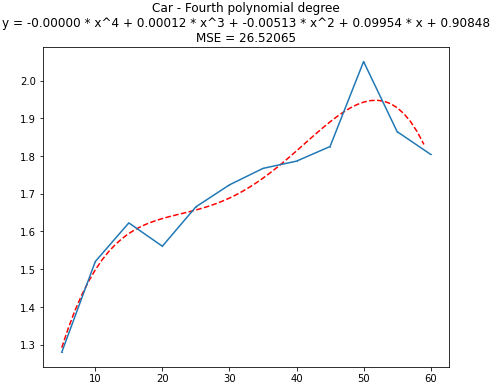
\includegraphics[width=1\linewidth]{Book/figures/6_approx_distancia/rectification2_lidar_car.png}
	\end{minipage}\hfill
	\begin{minipage}{0.32\textwidth}
		\centering
		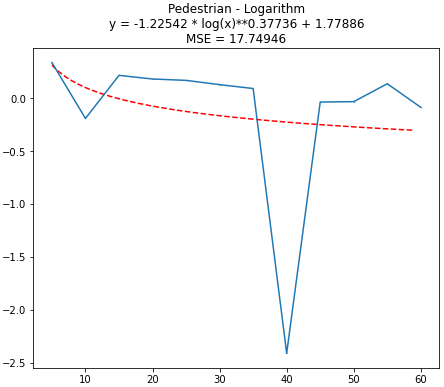
\includegraphics[width=1\linewidth]{Book/figures/6_approx_distancia/rectification2_lidar_pedestrian.png}
	\end{minipage}\hfill
	\begin{minipage}{0.32\textwidth}
		\centering
		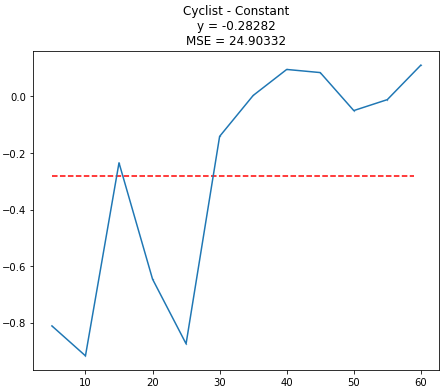
\includegraphics[width=1\linewidth]{Book/figures/6_approx_distancia/rectification2_lidar_cylist.png}
	\end{minipage}
	\caption{Modelo de rectificación de la distancia al centro de los objetos sin outliers.}
	\label{fig:Modelo de rectificación de la distancia al centro de los objetos sin outliers.}
\end{figure}

La Figura \ref{fig:Modelo de rectificación de la distancia al centro de los objetos sin outliers.} muestra los puntos calculados a partir de las medianas de las diversas regiones creadas en función de la distancia en la que se ha predicho la distancia a los objetos. Con estos puntos se han obtenido nuevas funciones a evaluar para intentar obtener funciones que se ajusten de mejor manera a los datos de validación sobre los que no se ha ajustado ningún modelo.

\begin{table}[H]
\centering
\begin{tabular}{|c|c|c|c|c|}
\hline
\textbf{Benchmark (MSE)} & \textbf{Fácil} & \textbf{Moderado} & \textbf{Difícil} & \textbf{Todo}\\ \hline \hline
Coche (distancia)        & 2,222          & 10,909             & 20,160       & 26,521     \\ \hline
Peatón (distancia)       & 5,467          & 13,691             & 18,198       & 17,912     \\ \hline
Ciclista (distancia)     & 6,404          & 18,799             & 29,000       & 24,903  \\ \hline
\end{tabular}
\caption{Evaluación del modelo de aproximación de distancia rectificado sin outliers.}
\label{fig:Evaluación del modelo de aproximación de distancia rectificado sin outliers.}
\end{table}

La evaluación obtenida tras el uso de las últimas funciones creadas sobre el dataset de validación no obtuvo los resultados esperados, ya que como se ve en la Figura \ref{fig:Evaluación del modelo de aproximación de distancia rectificado sin outliers.}, se empeoran las métricas en las clases 'coche' y 'ciclista', pero en la clase 'peatón' se consigue mejorar de forma muy sutil el \ac{MSE} sobre los datos de validación, por lo que la función ajusta sobre esta función es la utilizada finalmente.

Tras toda este serie de métodos para la obtención de la distancia en función de la nube se resume en los siguientes pasos:
\begin{enumerate}
    \item Proyección de la nube de puntos a las imágenes de la cámara.
    \item Filtrado la nube de puntos por cada bounding box 2D.
    \item Resolución de las intersecciones de los objetos 2D a partir de la obtención de la proximidad de los objetos, a partir del modelo basado en la altura de las cajas 2D, para así contabilizar los puntos del \ac{LiDAR} de las intersecciones en los objetos más cercanos a la cámara.
    \item Calculo de la distancia a los objetos, a partir de la mediana de la distancia a cada uno de los puntos de las bounding boxes 2D.
    \item Rectificación de la distancia aproximada a partir de las funciones de rectificación ajustadas.
\end{enumerate}

\section{Modelo de ensamble}
\label{sec:Modelo de ensamble}

En este punto se tienen dos modelos para la obtención de la distancia aproximada al centro de los objetos del entorno, siendo aquel basado en la altura de las bounding boxes 2D superior en precisión a aquel basado en la nube de puntos. Mientras que uno de los modelos es más estable en la mayoría de casos que se encuentran en el dataset, el otro mucho más preciso en casos sin ningún tipo de oclusión.

Debido a las diferentes fuentes de datos de las que provienen ambos modelos, se decide crear un modelo de ensamble que unifique los puntos fuertes de ambos modelos, para así obtener en conjunto un sistema mejorado que calcule de forma más precisa la distancia a los objetos. Se realiza tanto énfasis en este apartado, ya que cuanto mejor sea este sistema, más se puede reducir la \ac{RoI} que sea utilizada para la obtención de las detecciones 3D finales, además de reducir el tiempo de inferencia del modelo final basado en Deep Learning y nubes de puntos para la obtención de dichas detecciones finales por utilizar un espacio tridimensional menor).

El análisis del error de los modelos creados se decide realizar mediante el estudio de dos características por cada uno de los modelos, utilizándose para el modelo basado en la altura de las cajas 2D, la propia altura de la caja y la distancia que ha sido inferida, y por otra parte, en el caso del modelo basado en la nube de puntos del \ac{LiDAR} se estudiará el efecto del número de puntos sobre las bounding boxes 2D y la distancia aproximada por el propio modelo. De esta manera, va a ser necesario ajustar 4 funciones de error por cada una de las clases, lo que hacen 12 funciones diferentes para tratar de calcular los errores de ambos modelos y poder elegir de la mejor manera posible el modelo que puede calcular de forma más precisa la distancia a los objetos.

\begin{figure}[H]
    \centering
    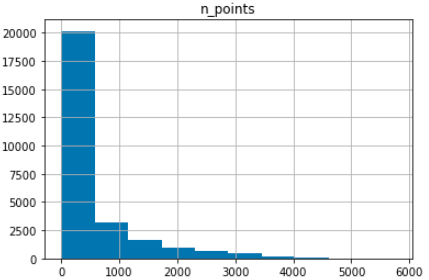
\includegraphics[width=0.4\textwidth]{Book/figures/6_approx_distancia/n_points_hist.png}
    \caption{Histograma con la cantidad de puntos sobre las bounding boxes 2D.}
    \label{fig:Histograma con la cantidad de puntos sobre las bounding boxes 2D.}
\end{figure}

Debido a que hasta ahora no se ha trabajado con la cantidad de puntos que se encuentran en las bounding boxes de los objetos, se muestra en la Figura \ref{fig:Histograma con la cantidad de puntos sobre las bounding boxes 2D.}, el histograma de la cantidad de puntos en los objetos de la parte frontal del vehículo. Se puede apreciar como la gran mayoría de objetos tienen muy pocos puntos del \ac{LiDAR}, pero pueden ascender hasta una cantidad superior a 5000 puntos lo cual indicaría que el objeto está muy cerca del vehículo y muy posiblemente sin oclusión ninguna (lo cual se ha visto con la muestra del dataset que esta premisa es cierta).

En el análisis de los errores de ambos modelos se ha planteado la creación de curvas que se ajusten a los errores cometidos de forma absoluta, todo ello en función de las característica definidas previamente además de las clases de los objetos analizados. Como primera aproximación se decide extraer por diferentes regiones el último decil para definir de esta manera los errores máximos producidos en esta región definida por las características estudiadas. De esta manera se tienen 'n' puntos iguales al numero de regiones por las que se calcula dicho decil, y a partir de estos puntos se puede ajustar una función que defina la relación entre la característica estudiada y el error cometido por el modelo, de manera que conocería cuando es mejor utilizar un modelo y cuando no.

Durante el ajuste de todas las funciones polinómicas definidas de grado 1 a grado 10, se encuentra con un problema de sobreajuste. Debido a que solo se está trabajando con los datos de entrenamiento para todos los análisis, excepto para la evaluación de la distancia final que se realiza con los datos de validación, se encuentra con que al ajustar los puntos que se han creado, se están obteniendo siempre funciones de un gran valor polinómico, como se ve en la Figura \ref{fig:Ajuste de las funciones de error de los modelos.} donde todos los puntos son perfectamente ajustados por las curvas creadas. El problema de dichas curvas perfectamente ajustadas se encuentra en los límites de todas las funciones, donde se empieza y termina con una gran pendiente, esto es producido por tanto a todos los grados de libertad por los que se han podido ajustar las funciones. Como solución a este problema, los puntos de validación de las curvas (pertenecientes también a los datos de entrenamiento) se han modificado para que también se encuentren antes del primer punto con el que se ajusta y también después del último punto de los usados para el ajuste de la curva.

La Figura \ref{fig:Ajuste de las funciones de error de los modelos sin overfitting.} muestra como este método de reducción del overfitting ha sido lo suficientemente efectivo para reducir la grado de la función ajustada además de los extremos de las función donde ya no se observa esas pendientes tan pronunciadas encontradas en la Figura \ref{fig:Ajuste de las funciones de error de los modelos.}. Tras la creación de estos funciones solo faltaría unir estos errores con algún tipo de fórmula que nos permita la selección de un modelo u otro para la obtención de una distancia más precisa, como se verá a continuación.

\begin{figure}[H]
	\begin{minipage}{0.32\textwidth}
		\centering
		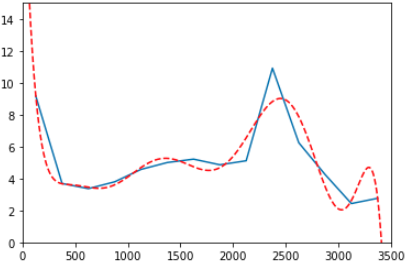
\includegraphics[width=1\linewidth]{Book/figures/6_approx_distancia/ensemble_overfitting_0.png}
	\end{minipage}\hfill
	\begin{minipage}{0.32\textwidth}
		\centering
		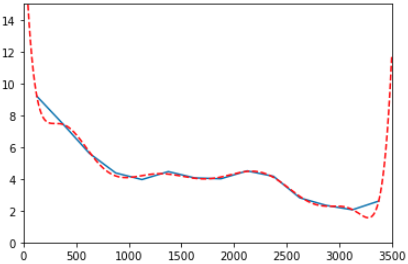
\includegraphics[width=1\linewidth]{Book/figures/6_approx_distancia/ensemble_overfitting_1.png}
	\end{minipage}\hfill
	\begin{minipage}{0.32\textwidth}
		\centering
		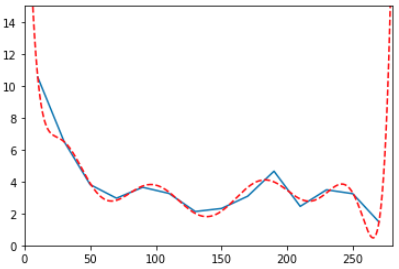
\includegraphics[width=1\linewidth]{Book/figures/6_approx_distancia/ensemble_overfitting_2.png}
	\end{minipage}
	\caption{Ajuste de las funciones de error de los modelos.}
	\label{fig:Ajuste de las funciones de error de los modelos.}
\end{figure}

\begin{figure}[H]
	\begin{minipage}{0.32\textwidth}
		\centering
		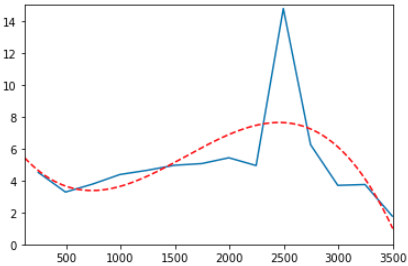
\includegraphics[width=1\linewidth]{Book/figures/6_approx_distancia/ensemble_not_overfitting_0.png}
	\end{minipage}\hfill
	\begin{minipage}{0.32\textwidth}
		\centering
		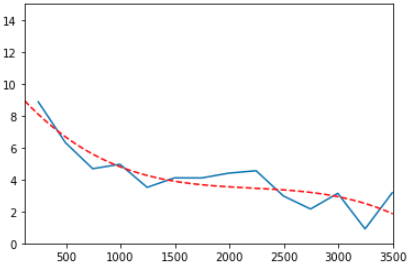
\includegraphics[width=1\linewidth]{Book/figures/6_approx_distancia/ensemble_not_overfitting_1.png}
	\end{minipage}\hfill
	\begin{minipage}{0.32\textwidth}
		\centering
		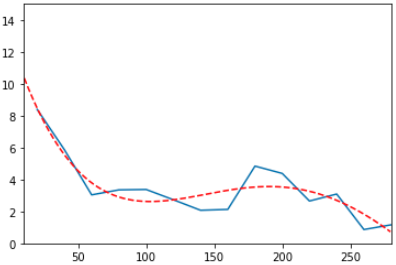
\includegraphics[width=1\linewidth]{Book/figures/6_approx_distancia/ensemble_not_overfitting_2.png}
	\end{minipage}
	\caption{Ajuste de las funciones de error de los modelos sin overfitting.}
	\label{fig:Ajuste de las funciones de error de los modelos sin overfitting.}
\end{figure}

Con las funciones que definen el error por cada una de las características, se decide realizar varias pruebas sobre el conjunto de datos de validación para observar si este modelo conjunto a conseguido algún tipo de mejora respecto de los que se tenían previamente, para ello se crean 4 fórmulas diferentes para dotar de peso a las salidas de los dos modelos que ya se tenían:

\begin{itemize}
    \item Selección de pesos basado en los deciles del error
    
    A partir de las funciones que obtienen el decil que define el 10\% de los peores errores a cometidos, se ejecuta por cada característica y tipo de objeto para con esto tener 2 puntuaciones por cada modelo en cada situación, de esta manera se definen los errores como $((error\_altura + error\_distancia\_altura) * distancia\_altura) * ((error\_n\_puntos + error_distancia\_nube\_puntos) * distancia\_nube\_puntos)$. El único problema es que la salida de las funciones que definen el error no suman 1, por lo que se proyectan dichos valores proporcionalmente para que la suma $error\_altura + error\_distancia\_altura + error\_n\_puntos + error_distancia\_nube\_puntos$ sea igual a 1.
\begin{table}[H]
\centering
\begin{tabular}{|c|c|c|c|}
\hline
\textbf{Benchmark (MSE)} & \textbf{Fácil} & \textbf{Moderado} & \textbf{Difícil}\\ \hline \hline
Coche (distancia)        & 2,137          & 6,499             & 8,618\\ \hline
Peatón (distancia)       & 1,916          & 2,802             & 3,430\\ \hline
Ciclista (distancia)     & 2,214          & 5,038             & 6,335\\ \hline
\end{tabular}
\caption{Evaluación del modelo ensemble utilizando los deciles de los errores.}
\label{tab:Evaluación del modelo ensemble utilizando los deciles de los errores.}
\end{table}

    \item Selección de pesos basado en los deciles del error cuadrático
    
    De la misma manera que se calculó el error en función de los parámetros analizados, se modifica el error del 10\% peor de los casos y se eleva al cuadrado para de esta manera obtener un modelo que perjudique aún más a los mayores errores, tras esto se proyectan los errores para que la suma de todos ellos sea igual a 1.
\begin{table}[H]
\centering
\begin{tabular}{|c|c|c|c|}
\hline
\textbf{Benchmark (MSE)} & \textbf{Fácil} & \textbf{Moderado} & \textbf{Difícil}\\ \hline \hline
Coche (distancia)        & 2,061          & 6,824             & 8,863\\ \hline
Peatón (distancia)       & 1,836          & 2,339             & 2,691\\ \hline
Ciclista (distancia)     & 2,007          & 4,26             & 4,834\\ \hline
\end{tabular}
\caption{Evaluación del modelo ensemble utilizando los deciles de los errores cuadráticos.}
\label{tab:Evaluación del modelo ensemble utilizando los deciles de los errores cuadráticos.}
\end{table}

    \item Selección de pesos basado en los centiles del error
    
    Otra de las opciones probadas, es el remplazo de las funciones ajustadas por los deciles, a ser ajustadas por los centiles del error, por lo que se tiene en cuenta el 1\% de los peores errores de las regiones analizadas para la generación de las curvas que definen los errores. Tras este paso se calculan los pesos de la misma manera que el primer modelo de ensamble probado.
\begin{table}[H]
\centering
\begin{tabular}{|c|c|c|c|}
\hline
\textbf{Benchmark (MSE)} & \textbf{Fácil} & \textbf{Moderado} & \textbf{Difícil}\\ \hline \hline
Coche (distancia)        & 3,011          & 6,608             & 6,972\\ \hline
Peatón (distancia)       & 1,786          & 2,327             & 2,757\\ \hline
Ciclista (distancia)     & 1,542          & 3,030             & 3,379\\ \hline
\end{tabular}
\caption{Evaluación del modelo ensemble utilizando los centiles de los errores.}
\label{tab:Evaluación del modelo ensemble utilizando los centiles de los errores.}
\end{table}

    \item Selección de pesos basado en los centiles del error cuadrático
    
    Como último modelo creado, se ha decidido calcular el cuadrado de las funciones de error que se basan en los centiles, para castigar de la mayor forma posible a aquel modelo que más probabilidad tenga de fallar en cada momento.
\begin{table}[H]
\centering
\begin{tabular}{|c|c|c|c|}
\hline
\textbf{Benchmark (MSE)} & \textbf{Fácil} & \textbf{Moderado} & \textbf{Difícil}\\ \hline \hline
Coche (distancia)        & 3,721          & 7,459             & 7,286\\ \hline
Peatón (distancia)       & 1,927          & 2,383             & 2,690\\ \hline
Ciclista (distancia)     & 1,540          & 2,611             & 2,631\\ \hline
\end{tabular}
\caption{Evaluación del modelo ensemble utilizando los centiles de los errores cuadráticos.}
\label{tab:Evaluación del modelo ensemble utilizando los centiles de los errores cuadráticos.}
\end{table}

\end{itemize}

Los resultados mostrados en las Tablas \ref{tab:Evaluación del modelo ensemble utilizando los deciles de los errores.}, \ref{tab:Evaluación del modelo ensemble utilizando los deciles de los errores cuadráticos.}, \ref{tab:Evaluación del modelo ensemble utilizando los centiles de los errores.} y \ref{tab:Evaluación del modelo ensemble utilizando los centiles de los errores cuadráticos.}, han superado con creces las expectativas, ya que solo analizando los datos de entrenamiento, ha sido posible mejorar en gran medida las métricas obtenidas en el modelo basado en la altura y en el basado en la nube de puntos (como se puede observar de forma comparativa con las Tablas \ref{tab:Evaluación sobre KITTI del modelo de aproximación de distancia basado en regresión.} y \ref{fig:Evaluación del modelo de aproximación de distancia rectificado.}). Entre todas las variaciones probadas sobre modelo de ensamble, se observa como aquellas que hacen uso de los centiles para ajustar as curvas de error, son aquellas que obtienen un error menor en las dificultades mayores sin perjudicar apenas la dificultad 'Fácil'. Observando los resultados obtenidos entre los modelos que hacen uso de los centiles se decide decantar por el modelo que no utiliza el error cuadrático.

\begin{table}[H]
\centering
\begin{tabular}{|ll|}
\hline
\multicolumn{2}{|c|}{\textbf{Errores}}       \\ \hline
\multicolumn{1}{|l|}{\textbf{1\%}}  & -4.809 \\ \hline
\multicolumn{1}{|l|}{\textbf{5\%}}  & -3.460 \\ \hline
\multicolumn{1}{|l|}{\textbf{50\%}} & -0.372 \\ \hline
\multicolumn{1}{|l|}{\textbf{95\%}} & 4.005  \\ \hline
\multicolumn{1}{|l|}{\textbf{99\%}} & 7.044  \\ \hline
\end{tabular}
\caption{Centiles del error del modelo final de la aproximación de la distancia.}
\label{tab:Centiles del modelo final de la aproximación de la distancia.}
\end{table}

En este punto se tiene completo todo el sistema de aproximación de la distancia a los objetos, pero falta obtener el rango de error en el que se mueve todo el modelo creado. Para ello se eliminan las detecciones mayores de 50 metros, ya que de normal no se tienen puntos del \ac{LiDAR} a esta distancia, y es muy difícil detectar objetos con el sistema de detección 3D de objetos tan lejanos. Con esto se observa en la Figura \ref{tab:Centiles del modelo final de la aproximación de la distancia.}, que los centiles de error del nuevo modelo se encuentran a muy poca distancia de error, por lo que se realiza la aproximación de que el 97\%-98\% de los casos se encuentra en un error en el rango de [-5, +5] metros, lo cual será muy útil para el modelo de detección de objetos 3D.

\section{Análisis del error con YOLOv5}
\label{sec:Análisis del error con YOLOv5}

Las evaluaciones de todo el proceso de ajuste de la distancia a los objetos ha sido producida sobre los datos del dataset, por lo que ningún tipo de error sobre las bounding boxes 2D ha sido probado sobre este sistema, para comprobar como funcionaría en el sistema de detección completo, se ha decidido aplicar el modelo YOLOv5m entrenado previamente para obtener las predicciones de dicho modelo, y utilizarlo para calcular el error a la distancia real utilizando las cajas 2D dadas por el modelo de detección 2D.

El problema de realizar este proceso de evaluación con las predicciones del modelo YOLOv5m es la asociación de las cajas 2D propuestas y el ground-truth del dataset, ya que es necesario calcular el \ac{IoU} ($\frac{Área\ de\ intersección}{Área\ de\ unión}$) de las cajas predichas sobre las reales para poder asociar a cada una, la que mejor se ajusta al ground-truth del dataset.

\begin{table}[H]
\centering
\begin{tabular}{|c|c|c|c|}
\hline
\textbf{Benchmark (MSE)} & \textbf{Fácil} & \textbf{Moderado} & \textbf{Difícil}\\ \hline \hline
Coche (distancia)        & 3.296          & 7.349             & 7.072\\ \hline
Peatón (distancia)       & 2.030          & 2.417             & 2.807\\ \hline
Ciclista (distancia)     & 2.207          & 3.787             & 3.803\\ \hline
\end{tabular}
\caption{Evaluación del modelo ensemble sobre las detecciones obtenidas del modelo YOLOv5m.}
\label{fig:Evaluación del modelo ensemble sobre las detecciones obtenidas del modelo YOLOv5m.}
\end{table}

Tras realizar todo el cálculo de la asociación, se aplica todo el modelo de aproximación de la distancia y se evalúa todas las distancia a los objetos ya que las cajas 2D, ya que han sido modificadas y no son iguales a los datos con los que se trabaja en el dataset. Los resultados obtenidos son similares a los vistos previamente como se puede observar en la Figura \ref{fig:Evaluación del modelo ensemble sobre las detecciones obtenidas del modelo YOLOv5m.}, aunque se mejora ligeramente en la métrica de los coches. Esto puede ser debido a que muchas detecciones del modelo son eliminadas si no superan un \ac{IoU} del 70\%, como se indica en el dataset de KITTI, ya que en este caso se considerarían como detecciones incorrectas.